% !BIB program=biber
\documentclass[scheme=chinese,a4paper]{article}
\usepackage[utf8]{inputenc}
\usepackage{amsmath}
\usepackage{esint}
\usepackage{tabstackengine}
\usepackage{xeCJK}
\usepackage{caption}
\usepackage{stackengine}
\usepackage{graphicx}
\graphicspath{ {./figure/} }
\usepackage{float}
\usepackage{amsmath}
\usepackage{ulem}
\usepackage{amsfonts}
\usepackage{xcolor}
\usepackage{tikz}
\usetikzlibrary{calc}
\usepackage{pgfplots}
\usepackage{mathrsfs}
\usepackage{listings}
\lstset{basicstyle=\ttfamily\footnotesize,breaklines=true}
\usepackage{url}
\usepackage[colorlinks,linkcolor=black]{hyperref}
\usepackage{enumitem}
\setlist[1]{itemsep=-5pt}
\usepackage{subcaption}
\usepackage{pdfpages}
\usepackage{booktabs}
\usepackage{multirow}
\usepackage[toc,page]{appendix}
\usepackage{geometry}
\usepackage{fancyhdr}
\usepackage{lipsum}
\usepackage{type1cm}
\usepackage{caption}
\usepackage{subcaption}


\geometry{a4paper,top=3.1cm,bottom=1cm} %设置留白
\newcommand{\song}{\CJKfamily{song}}
\fontsize{12pt}{22pt}\selectfont
%\setlength{\baselineskip}{30pt}  %设置行间距

\usepackage[backend=biber,style=gb7714-2015]{biblatex} 
\addbibresource{../resources/bibs/refs.bib}

\usetikzlibrary{shapes,arrows}
\usetikzlibrary{arrows}

%%%% 下面的命令重定义页面边距,使其符合中文刊物习惯 %%%%
\addtolength{\topmargin}{-54pt}
\setlength{\oddsidemargin}{0.63cm}  % 3.17cm - 1 inch
\setlength{\evensidemargin}{\oddsidemargin}
\setlength{\textwidth}{14.66cm}
\setlength{\textheight}{24.00cm}    % 24.62

%%%% 段落首行缩进两个字 %%%%
\makeatletter
\let\@afterindentfalse\@afterindenttrue
\@afterindenttrue
\makeatother
\setlength{\parindent}{2em}  %中文缩进两个汉字位

%%%% 下面的命令设置行间距与段落间距 %%%%
\linespread{1.4}
% \setlength{\parskip}{1ex}
\setlength{\parskip}{0.5\baselineskip}

%%%% 重定义 %%%%
\renewcommand{\contentsname}{目录}  % 将Contents改为目录
\renewcommand{\abstractname}{摘要}  % 将Abstract改为摘要
\renewcommand{\refname}{参考文献}   % 将References改为参考文献
\renewcommand{\indexname}{索引}
\renewcommand{\figurename}{图}
\renewcommand{\tablename}{表}
\renewcommand{\appendixpagename }{附录}
\renewcommand{\appendixtocname }{附录}
% \renewcommand{\algorithm}{算法}
% Turn on the style
%\pagestyle{fancy}
%\fancyfoot{}
% Clear the header and footer
%\fancyhead{}

\pagestyle{fancy} % Turn on the style
\fancyhf{} % Start with clearing everything in the header and footer
% Set the right side of the footer to be the page number
\fancyfoot[R]{\thepage}
\fancypagestyle{plain}{%
    \fancyfoot[R]{\thepage}%
}

\renewcommand{\headrulewidth}{0pt}

\begin{document}
\begin{abstract}

  

本系统可实现终端一键启动,本队采用两块树莓派单板计算机分别作为两个摄像头的处理器,
调用OpenCV计算机视觉库对 OmniVision OV5647 摄像头所采集的信息进行图像处理。
基于高斯混合算法 (Mixture of Gaussians, MOG) 实现对图像的前景背景分离,进而对运动的
激光笔进行检测.。
通过以太网交换机进行流式视频传输以及数据交换, 创新性地使用了基于Web的交互平台搭建, 
可以精确测量柔性透明细线的长度 $l$ 与激光笔的平面摆动角度$\theta$。\\
\textbf{关键词:}单目标追踪、高斯混合算法、OpenCV、Web、物联网
\end{abstract}

\section{设计任务与要求}
\begin{figure}[H]
    \centering
    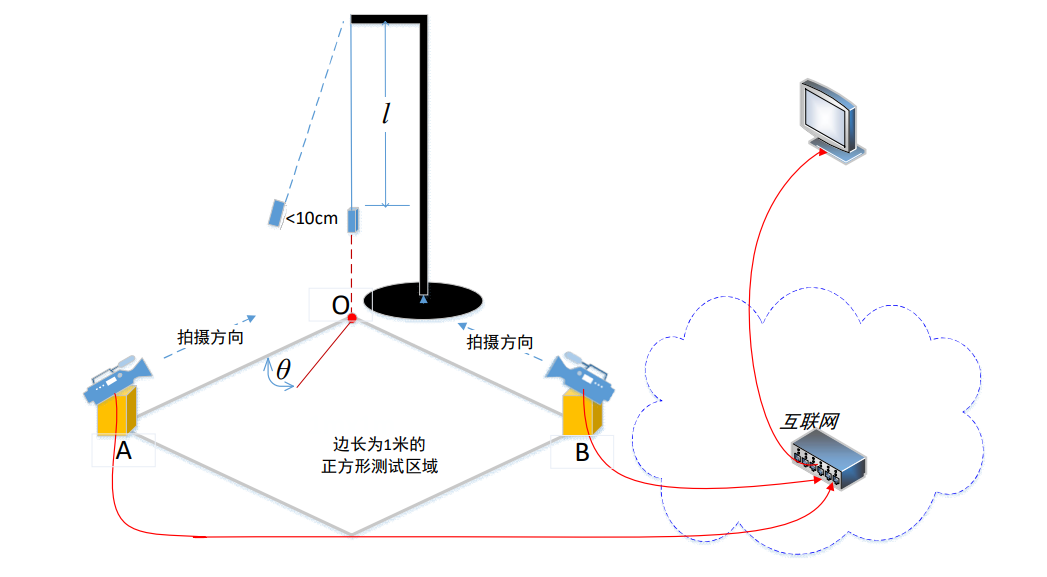
\includegraphics[width=1\textwidth]{3.png}
    \caption{系统框图}
\end{figure}
本系统的主要研究内容包括以下方面:

\begin{enumerate}
  \item 激光笔运动轨迹的捕捉以及显示。
  \item 测量柔性透明细线的长度 $l$与激光笔的平面摆动角度$\theta$。
\end{enumerate}

\section{方案设计与论证}
本系统采用两块树莓派微型单板计算机分别作为两个摄像头的处理器,
利用树莓派强大的性能,使用相机串行接口 (Camera Serial Interface, CSI) 摄像头,
使用 Python 调用OpenCV计算机视觉库对摄像头所采集的信息进行处理,
采用MOG2算法将前景背景分离开来, 对前景物体进行追踪, 从而得到物体的运动轨迹。
用单摆近似公式,通过识别测量摆动周期$T$,计算得到摆长,即细线长度$l$。
利用三角形正切公式,通过识别测量$A$、$B$两点画面中单摆横轴方向的振幅,计算得到角度$\theta$。
使用 HTTP 流式传输协议将树莓派所采集的图像发送至终端节点从而实现数据交换,
终端节点通过拉升GPIO的电平控制蜂鸣器发出声音,点亮小灯并在Web交互界面显示所需参数。
利用 systemd 进行服务管理以及进程守护, 从而得以顺利一键启动。

\subsection{MCU 选型}

\paragraph{方案一 OpenMV} OpenMV是一款自带了摄像头的基于 STM32 的模块,
OpenMV搭载MicroPython解释器,这允许我们在嵌入式上使用Python来编程 ,还可以通过UART,I2C,SPI以及GPIO等控制其他的硬件。
从而对摄像头采集到的信息进行图像处理,但不适合复杂的算法:比如OCR识别,车牌识别,
猫狗分类,深度学习之类的。

\paragraph{方案二 树莓派}
树莓派 (Raspberry Pi) 作为一款成熟的SOC, 其拥有丰富的外设扩展以及数量惊人的软件选择, 更重要的是其基于 Linux 的
Raspbian OS, 可以做到共享 \lstinline{x86} 平台的软件生态。 
考虑到本题的题目要求要求对采集图像时时显示,数据处理量较大,灵敏度要求较高,
选择树莓派作为 MCU。 

\subsection{目标跟踪}
本题难点在于对物体 (激光笔) 进行单目标跟踪, 本小组对以下几种单目标追踪算法进行了比较。

\paragraph{方案一Kalman滤波}
该算法需要建立物体的运动模型,
其服从高斯模型,来对目标状态进行预测,然后与观察模型进行比较,
根据两者之间的误差来寻找运动目标的状态, 
但其高斯运动模型在现实生活中很多条件下并得不到满足,
并且该算法对杂乱的背景也很敏感。Kalman 滤波属于生成类算法, 
即在当前帧对目标区域建模,下一帧寻找与模型最相似的区域就是预测位置。
\paragraph{方案二 Meanshift}
又称为均值漂移算法,是一种基于概率密度分布的跟踪方法,
使目标的搜索一直沿着概率梯度上升的方向,
迭代收敛到概率密度分布的局部峰值上。
即利用Meanshift算法可以快速找到领域目标最相似的
地方。但当目标速度较快时,跟踪效果不好;当目标尺度有所变化时,跟踪就会失败。 
\paragraph{方案三 高斯混合模型}
高斯混合模型 (Mixture of Gaussians, MOG) 是一种基于背景减法(也称为前景检测)的单目标追踪算法,
采用的是自适应的高斯混合模型,MOG2根据不同输入场景自动选择分量的个数,
它为每一个像素选择一个合适数目的高斯分布。
这样就会对由于亮度等发生变化引起的场景变化产生更好的适应。
在前景连续性及运算时间上具有较好的特性。

考虑到本题的题目要求要求对采集图像实时显示,同时可能存在背景干扰,
需要识别的物体在运动,变化情况多,于是选用方案三。

\section{理论分析与计算}

\subsection{图像识别工具}
图像识别的核心是图像的处理和识别,支持RPI摄像头,通过调运了OpenCV库,OpenCV是
Intel开源计算机视觉库。它由一系列 C 函数和少量 C++ 类构成,
实现了图像处理和计算机视觉方面的很多通用算法。开源且可以应用于工程实践中。
\subsection{透明细线长度$l$的计算}
运动中的激光笔近似在做单摆运动,借助 OpenCV 的库函数对视频中摆动
的激光笔进行识别,获取激光笔的位置信息,并对数据进行自动分析和计算。
\begin{figure}[H]
  \centering
  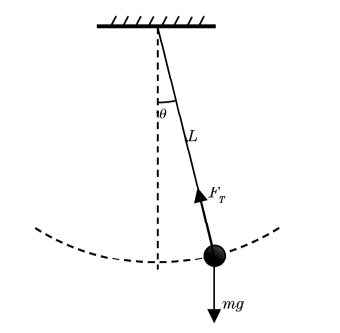
\includegraphics[width=0.3\textwidth]{7.png}
  \caption{单摆模型}
\end{figure}
数学关系如下:
根据牛顿第二定律,单摆的切向运动公式:
\begin{equation}
  -mg\cdot\sin\theta =m \cdot \frac{\mathrm{d}}{\mathrm{d}t^2}{\theta^2} L
\end{equation}
其中,m为摆球质量,L为摆线有效长度。整理得:
\begin{equation}
  \frac{\mathrm{d}}{\mathrm{d}t^2}{\theta^2} +\frac{g}{L}=0
\end{equation}
又因为
$\omega=\sqrt{\frac{L}{g}}$,
$T=2\pi\frac{L}{g}$
可得
\begin{equation}
  L=\frac{T^{2}}{4\pi^{2}}\cdot g
\end{equation}
\subsection{轨迹与 $OA$ 边的夹角$\theta$计算}
轨迹与 $OA$ 边的夹角为$\theta$,同样可以借助 OpenCV 的库函数对视频中摆动
的激光笔进行识别,获取激光笔的位置信息,并对数据进行自动分析和计算。

\begin{figure}[H]
    \centering
    \begin{subfigure}[b]{0.3\textwidth}
      \centering
      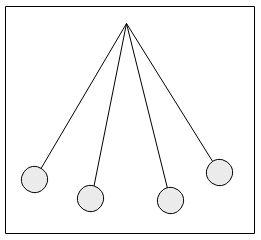
\includegraphics[width=\textwidth]{a}
      \caption{摄像头捕捉到的画面如图,激光笔在平面内单摆运动\\}
      \label{fig:y equals x}
    \end{subfigure}
    \hfill
    \begin{subfigure}[b]{0.3\textwidth}
      \centering
      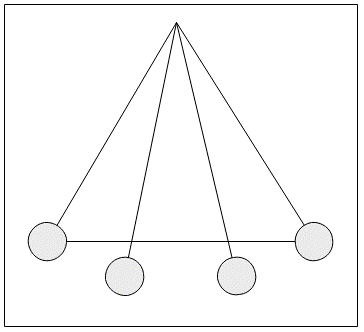
\includegraphics[width=\textwidth]{b}
      \caption{将激光笔到达两侧的最高点连接\\}
      \label{fig:three sin x}
    \end{subfigure}
    \hfill
    \begin{subfigure}[b]{0.3\textwidth}
      \centering
      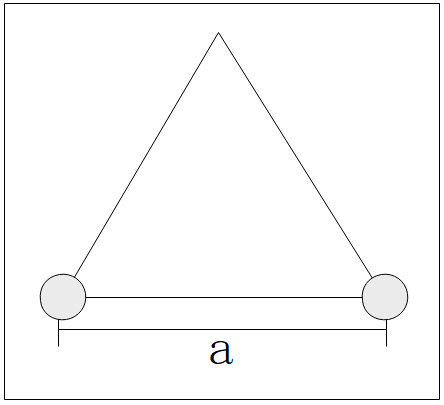
\includegraphics[width=\textwidth]{c}
      \caption{已知视频画面的分辨率,根据比例,求得$a$的大小\\}
      \label{fig:five over x}
    \end{subfigure}
      \caption{$OA$向摄像头拍摄画面}
      \label{fig:three graphs}
\end{figure}

\begin{figure}[H]
  \centering
  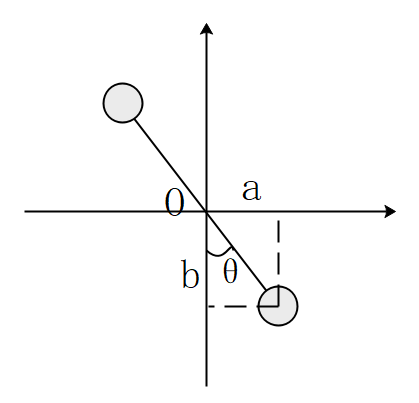
\includegraphics[width=0.4\textwidth]{9.png}
  \caption{俯视图}
\end{figure}
同理,可求得$b$的大小,由俯视图可知$\theta=\arctan{\frac{b}{a}} $,即可求出$\theta$。


\section{系统设计}
\subsection{硬件架构}
\begin{figure}[H]
  \centering
  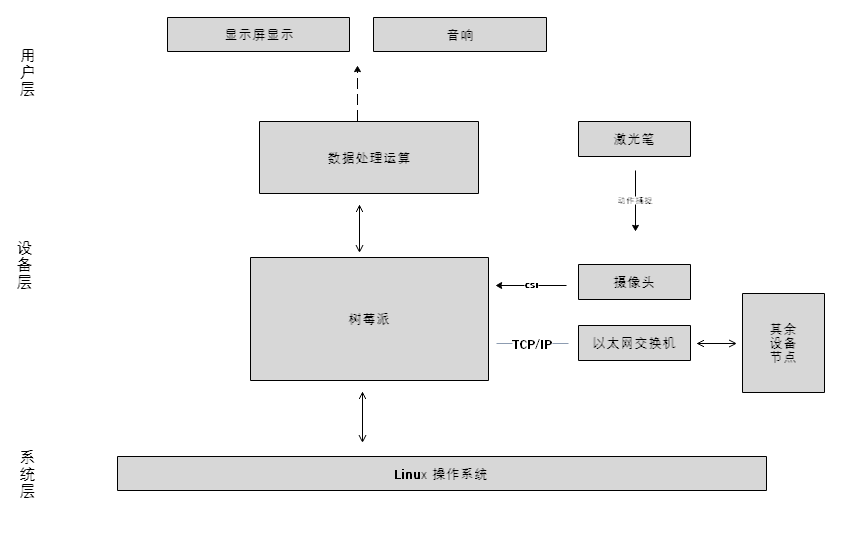
\includegraphics[width=1\textwidth]{sys.png}
  \caption{系统层次框图}
\end{figure}
本系统使用树莓派作为系统的核心部分, 两块树莓派作为摄影节点, 将图像进行初步识别后经由 HTTP 协议
发送至终端节点. 系统架构采用客户端-服务器模式, 终端节点作为客户端对摄像节点 (即服务器) 进行
轮询请求. 终端节点将服务器请求得到的数据进行清洗和滤波等复杂计算, 最后利用 JavaScript 脚本
操作 DOM 的能力将结果展示给用户. 

该系统的优点在于其终端节点的选择灵活性高, 只要搭载着可以运行浏览器的设备, 就可以作为终端节点. 
同时也充分利用了摄影节点的性能, 减轻计算负担, 提高整套系统的性能效率. 但缺点在于逻辑实现较为
复杂, 需要设计良好的应用程序借口 (API) 以进行数据的传输, 同时对网络带宽要求高. 

\subsection{界面以及用户体验设计}
\begin{figure}[H]
  \centering
  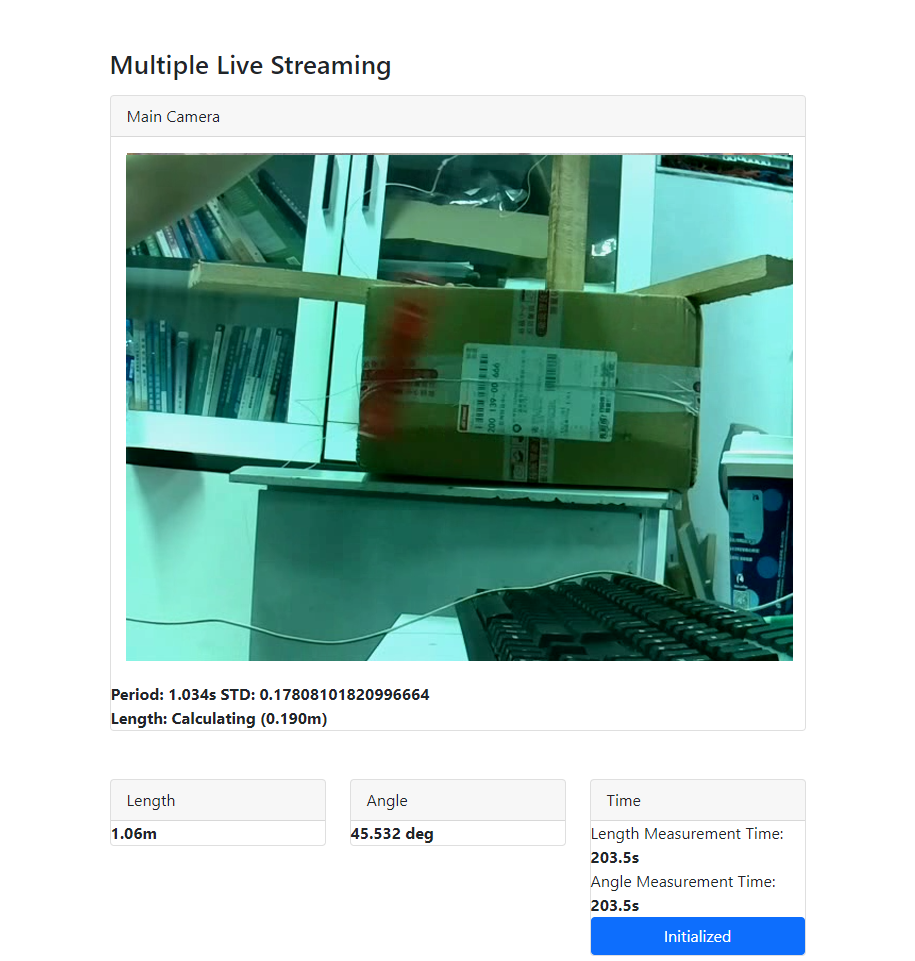
\includegraphics[width=0.8\textwidth]{interface.png}
  \caption{测量界面示意图}
\end{figure}

本系统的用户交互界面使用了 Bootstrap 前端框架作为元件素材库, 提供字体排印、
窗体、按钮、导航及其他各种组件及Javascript扩展,旨在使动态网页和Web应用的开发更加容易。
Bootstrap还包括了其他常用的界面元素,例如带有高级功能的按钮(例如按钮组合、带有下拉菜单选项
的按钮、导航栏、水平和垂直标签组、导航、分页等等)、标签、高级排版、缩略图、警告信息、进度条等。
这些组件都使用CSS的类实现。在页面中需要将其对应到特定的HTML元素上面。

摄像节点捕捉到的画面可以实时显示在画面的左右两侧, 在其下可以看到测量数据的标准差, 长度以及计算的角度. 
当角度或者长度计算完成时, 终端节点会通过扬声器发出声音提示, 同时右下角会显示「成功」字样并且出现绿色的
图像提示. 同时还显示测量角度以及长度的所需时间, 所有信息一目了然. 

\section{系统测试及结果}
\subsection{测试仪器}

\begin{table}[H]
  \centering
  \caption{测试仪器}
    \begin{tabular}{ccc}
    \toprule
    \multirow{1}[2]{*}{仪器名称} & \multirow{1}[2]{*}{型号规格} & \multirow{1}[2]{*}{数量}\\
  
    \midrule
    关节角度测量尺    &  $180^\circ$  & 1\\
    \midrule
    显示屏   &   24寸    & 3\\
    \midrule
    卷尺    &  3m  & 1   \\
    \midrule
    秒表    &  电子式  & 1   \\
    \bottomrule
    \end{tabular}%
\end{table}%
\subsection{测试方法}
\begin{enumerate}
  \item 视频显示,使激光笔做单摆运动,摄像头记录采集,在终端显示屏观察其采集到的激光笔运动画面。
  \item 启动时,按下秒表计时,测量完成时,观察终端声光提示及秒表时间,
  比较屏幕显示的细线长度与细线实际长度、计算所得夹度与初始测量角度。
\end{enumerate}

\subsection{性能指标}
\subsubsection{基础指标}
\begin{enumerate}
  \item 测量系统在终端节点设置一键启动,开启系统。
  \item 能够识别激光笔,并用红色方框标出。
  \item 分别显示两个摄像头拍摄到的激光笔的运动视频。
  \item 测量激光笔运动轨迹与 $OA$ 边的夹角为$\theta$,测量透明细线长度 $l$。
  \item 测量完成时,终端声光提示并显示长度 $l$(50cm$\leq l \leq$≤150cm)。
\end{enumerate}
\subsubsection{提升指标}
\begin{enumerate}
  \item 一键启动后,当 $\theta=0^{\circ}$ 和 $\theta=90^{\circ}$时,能自动测量长度 $l$,50cm$\leq l\leq$150cm。
要求测量误差绝对值小于 2cm, 测量时间小于 30 秒。
  \item 一键启动后,可以测量 $\theta \leq 0^\circ$和$\leq \theta \leq 90^\circ$。要求测量误差绝对值小于$5^\circ$。 测量时间小于 30 秒。
\end{enumerate}

测试结果见附录

\section{总结}
本系统能够在终端节点一键启动,启动后显示两个摄像节点拍摄到激光笔的运动视频,
在规定时间内完成测量,测量完成时,终端声光提示并显示长度 $l$ 和角度$\theta$。较好的满足题目要求。
测试中发现系统在显示激光笔运动视频是有延迟,
分析原因是由于网络发生了丢包,
解决方案是采用降低摄像头分辨率及帧数从而达到减少网络丢包的目的。
\begin{thebibliography}{5}  
\bibitem{ref1}目标跟踪入门篇-相关滤波[N],微信公众号:计算机算法学习工程师,2021-07-05(1) 
\bibitem{ref2}郭莉,在统计分析中如何识别极端值[J],统计学,期刊网,1999(11),19-20
\bibitem{ref3}黄膺达,王旗,基于图像处理的单摆测量重力加速度实验的研究[J],中国知网,2020(05),14-17
\bibitem{ref4}胡亮,杨德贵,王行,廖祥红,基于改进MEANSHIFT的可见光低小慢目标跟踪算法[J],中国知网,2021(1),1-14
\bibitem{ref5}董谱,张国平,刘燕,汪馨童,杨晓霞,基于以太网和OpenCV的仓库监控系统设计[J],中国知网,2021(10),22-27

\end{thebibliography}
\begin{appendices}

\begin{table}[H]
  \centering
  \caption{基础题测试结果}
    \begin{tabular}{ccc}
    \toprule
    \multirow{1}[2]{*}{测试内容} & \multirow{1}[2]{*}{测试结果} & \multirow{1}[2]{*}{是否满足测试要求}\\
    
    够识别激光笔,并用红色方框标出   &   成功识别并标出    & 是\\
    \midrule
    实时分别显示两个摄像头拍摄到的激光笔的运动视频    &  成功分别显示  & 是  \\
    \midrule
    测量完成时,终端声提示    &  音箱发出提示音  & 是   \\
    \midrule
    测量完成时,显示长度$l$    &  显示长度$l$  & 是   \\
    \midrule
    测量所需时间    &  小于30s  & 是   \\
    \bottomrule
    \end{tabular}%
\end{table}%
\begin{table}[H]
  \centering
  \caption{提升题测试结果}
    \begin{tabular}{ccc}
    \toprule
    \multirow{1}[2]{*}{测试内容} & \multirow{1}[2]{*}{测试结果} & \multirow{1}[2]{*}{是否满足测试要求}\\
    \midrule
    $\theta$等于$90^\circ$时,测量长度$l$    &  测出长度$l$,且误差绝对值小于2cm,测量时间小于30s  & 是\\
    \midrule
    $\theta$等于$90^\circ$时,测量长度$l$    &  测出长度$l$,且误差绝对值小于2cm,测量时间小于30s  & 是\\
    \midrule
    测量 $\theta$角度   &  测出角度$\theta$,且误差绝对值小于$5^\circ$,测量时间小于30s  & 是  \\
    \bottomrule
    \end{tabular}%
\end{table}%


\begin{table}[htbp]
  \centering
  \caption{长度以及角度}
  \begin{tabular}{cccccc}
  \hline
    绳长$l$/cm & $\theta$/deg & \multicolumn{4}{c}{估计长度$\hat{l}$/cm}  \\ 
    \hline
    60 & 0 & 58.9 & 61.3       & 59.5 & 60.3 \\
    90 & 0 & 91.2 &  90.5       & 89.6        & 89.2   \\
    110 & 0 & 109.0 &  110.5       & 111.6        & 109.2   \\
    60 & 90 & 59.9 & 60.4        & 58.7 & 60.9 \\
    90 & 90 & 90.7 &  91.5       & 88.6        & 88.2   \\
    110 & 90 & 109.2 &  110.7       & 111.5        & 109.5   \\
    \hline
  \end{tabular}
\end{table}

\begin{table}[htbp]
  \centering
  \caption{具体测试角度$\theta$数据}
  \begin{tabular}{cp{0.5cm}p{0.5cm}p{0.5cm}p{0.5cm}}
  \hline
    $\theta$/deg & \multicolumn{4}{c}{测量数据$\hat{\theta}$/deg}  \\ \hline
    30 & 33 & 32 & 33 & 29 \\
    55 & 55 &  57       & 54        & 51   \\
    75 & 72 &  72       & 74        & 76   \\\hline
  \end{tabular}
\end{table} 

\end{appendices}
\end{document}